\chapter{Założenia projektowe}
\label{cha: zalozeniaprojektowe}

Głównym założeniem tej pracy inżynierskiej było wykonanie strzeleckich ochronników słuchu. Zamysł był wzorowany na istniejących produktach, choć miał rozszerzać ich funkcjonalność. Słuchawki miały składać się z materiału tłumiącego, elektronicznego układu przetwarzania dźwięku z otoczenia oraz złącza do komunikacji radiowej. Elektroniczny układ spełniał główne zadanie w słuchawkach, ponieważ przekazywał dźwięk z otoczenia oraz z radiotelefonu do ucha użytkownika, aby materiał tłumiący nie zakłócał normalnej komunikacji oraz dokonywał aktywnego wyciszenia dźwięków, podobnie jak w słuchawkach multimedialnych, kiedy natężenie fali akustycznych przekraczało określony poziom.

Słuchawki miały być stworzone od podstaw aż do otrzymania gotowego produktu, co obejmowało:

\begin{itemize}
	\item dobór parametrów głośników, mikrofonów, baterii i innych elementów
	\item zaprojektowanie, zamówienie i zlutowanie płytki PCB
	\item napisanie oprogramowania do mikrokontrolera przetwarzającego sygnały
	\item zaprojektowanie i wydrukowanie na drukarce 3D obudowy słuchawek
	\item dobór materiału tłumiącego pasywnie
\end{itemize}

Głównym ograniczeniem dla projektu było przetworzenie sygnału od mikrofonu do głośnika w identycznym czasie, w jakim tę drogę pokona fala dźwiękowa, aby idealnie nałożyć na nią antyfazę. Przy prędkości dźwięku wynoszącej $ 331,3m/s $\ref{cha:dwiek}, pokonanie $1cm$ zajmuje fali akustycznej $29,16\mu s$. Prędkość sygnału elektrycznego jest pomijalna, ponieważ wynosi 1/3 prędkości światła. Istotna była natomiast szybkość konwersji przetworników, które wprowadzają do układu największe opóźnienia.

Na schemacie \ref{pic:conv_time} przedstawiono poglądowo równoległy przepływ sygnału cyfrowego oraz analogowego.

\begin{figure}[H]
	\centering
	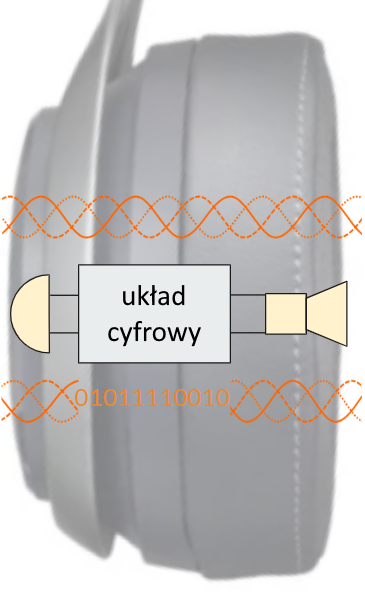
\includegraphics[height=6cm]{zdjecia/conv_time.png}
	\caption{\label{pic:conv_time} Schemat poglądowy równoległego przepływu dźwięku}
\end{figure}



\chapter{Istniejące rozwiązania}
\label{cha:ist_rozw}

\textbf{JAK DZIAŁAJĄ TAKIE SORDINY}